\documentclass[ ../main.tex]{subfiles}

\SetKwFunction{MakeSingularHashSet}{make\_singular\_hash\_set}
\SetKwFunction{Encode}{encode}
\SetKwFunction{trunc}{tr}
\SetKwFunction{shs}{shs}
\SetKwData{SHS}{SHS}

\SetKwData{Btm}{0}
\SetKwData{Top}{1}

\providecommand{\mainx}{..}

\begin{document}
\section{The \emph{Singular Hash Set}}
\label{sec:shs}
We would like to have properties of both homomorphisms $\Fun{F}$ and $\Fun{G}$ but with a much smaller space complexity.

In what follows, we provide a theoretical implementation of the \emph{cipher set} that obtains optimality in the following ways:
\begin{enumerate}
	\item The space complexity obtains the theoretical lower-bound of a random approximate positive set with an expected false positive rate $\fprate$.
	\item The entropy obtains the upper bound for the given expected space complexity.
\end{enumerate}

\begin{definition}
\label{alg:makeset}
	The \emph{data type} for the \emph{cryptographic} singular hash set is defined as $\SHS_{\Fun{F} \Set{X}} \coloneqq \BitSet^k \times \BitSet^*$ with a value constructor $\shs_{\Fun{F}\Set{X}} \colon \PS{\Set{X}} \times \SetBuilder{2^{-k} \in \RatSet}{k \in \NatSet} \mapsto \SHS_{\Fun{F} \Set{X}}$ defined as
	\begin{equation}
	\shs_{\Fun{F} \Set{X}}(\Set{A}, \fprate) \coloneqq \Tuple{q,n'}
	\end{equation}
	where
	\begin{equation}
	\begin{split}
	\Set{A}     & = \{x_{(1)},\ldots,x_{(m)}\}\,,\\
	k			& \coloneqq -\log_2 \fprate\,,\\
	\hash_k(b,n)& \coloneqq \trunc\left(\hash\left(b \cat n'\right),k\right)\,,\\	
	\phi(w,n) 	& \coloneqq \hash_k\left(\Fun{E}(w), n\right)\,,\\
	\Omega_l 	& \coloneqq \SetBuilder{\phi(x,l) \in \BitSet^k}{w \in \Fun{F}(\Set{A})}\,,\\
	n 			& \coloneqq \min\SetBuilder{ j \in \NatSet }{ \Omega_j \in \PS{\BitSet^k} \land \Card{\Omega_j} = 1}\,,\\
	q 			& \coloneqq \phi\left(\Fun{F} x_{(1)},n\right)\,.
	\end{split}
	\end{equation}
where $\Fun{F} \colon \Set{X} \mapsto \Set{W}$ is a homomorphism and $\Fun{E} \colon \Set{W} \mapsto \BitSet^*$ is a prefix-free coder.\footnote{If $\Fun{E}$ is not prefix-free, then an approximation error independent of parameter $\fprate$ is introduced.}
\end{definition}
%TODO: randomly sample from a population of bit strings that have the same floor log n.

If $\Fun{F}$ is the \emph{identify} function $\Fun{id} \colon \Set{X} \mapsto \Set{X}$ then the singular hash set models a random approximate positive set over $\Set{X}$, denoted by $\PAT{\left(\PS{\Set{X}}\right)}$.
However, typically, the singular hash set is intended to be used for as a \emph{cipher set}, a parametric type $\PAT{\OTL{\OT{\Set{X}}}}$ where $\Fun{F} \colon \Set{X} \mapsto \OT{\Set{X}}$, e.g., $x \overset{\Fun{F}}{\mapsto} \OT{x}$ where $\OT{x}$ may be, say, an \emph{equivalence class} $\{\OT{x}_1,\ldots,\OT{x}_k\}$ in which each of the elements map back to $x$ under $\Fun{F}^{-1} \colon \OT{\Set{X}} \mapsto \Set{X}$.

\begin{theorem}
The data type $\SHS$ with value constructor $\shs \colon \PowerSet(\BitSet^*) \times \SetBuilder{2^{-k} \in \RatSet}{k \in \NatSet} \mapsto \SHS$ over the computational basis $\SetContains \colon \SHS \times \BitSet^* \mapsto \BitSet$ is a random approximate positive set of $\OT{\Set{A}}$ with a \emph{false positive rate} $\fprate$ over $\OT{\Set{X}} \SetDiff \OT{\Set{A}}$.
That is, \emph{a priori},
\begin{equation}
	\shs_{\Set{X}}(\Set{A},\fprate) \sim \PAT{\OT{\Set{A}}}[\fprate]
\end{equation}
for any $\Set{A} \in \PS{\Set{X}}$ and $\fprate \in \SetBuilder{2^{-k} \in \RatSet}{k \in \NatSet}$.
\end{theorem}
\begin{proof}
In order for the value $\shs_{\Set{X}}(\Set{A},\fprate)$ to be a random approximate set with a distribution given by $\PAT{\OT{\Set{A}}}[\fprate]$, it must satisfy two conditions as specified by \cref{def:approx_set}:
\begin{enumerate}
	\item $\OT{\Set{A}}$ is a subset of $\PAT{\OT{\Set{A}}}$.
	This condition guarantees that no \emph{false negatives} may occur.
	\item An element in $\OT{\Set{X}}$ that is not a member of $\OT{\Set{A}}$ is a member 
	of $\PAT{\OT{\Set{A}}}$ with a probability $\fprate$, denoted the false positive rate, 
	i.e.,
	\begin{equation}
	\Prob{x \in \AT{\OT{\Set{A}}} \Given x \notin \OT{\Set{A}}} = \fprate
	\end{equation}
	for any $x \in \Set{X}$.
\end{enumerate}

To prove the first condition, note that \cref{alg:contains} tests any element $x$ for membership in $\PASet{S}$ by computing the hash of $x$ concatenated with the bit string $b_n$ and returning \True if the hash is $h_k$ where \cref{alg:makeset} finds bit strings $b_n$ and $h_k$ such that each element of $\Set{S}$ concatenated with $b_n$ hashes to $h_k$.

To prove the second condition, suppose we have a set $\Set{S} = \{x_1,\ldots,x_m\}$ and each element in $\Set{S}$ hashes to $y = \hash(x_1)$. By \cref{asm:ro_approx}, $\hash \colon \BitSet^* \mapsto \BitSet^k$ approximates a random oracle and thus uniformly distributes over its domain of $2^k$ possibilities. Since $y$ is a particular element in $\BitSet^k$, the probability that an element not in $\Set{S}$ hashes to $y$ is $2^{-k}$.
\end{proof}




In particular, we consider a data type that supports both the membership and identity relations while obtaining the information-theoretic expected lower-bound for space with respect to the false positive rate.
Since it obtains the information theoretic lower-bound, the bit strings generated naturally obtain \emph{maximum entropy}, i.e., any set $\Set{A} \in \PS{\Set{X}}$ a priori maps to random bit string in its representation.
The only information it leaks is related to its expected bits per element, i.e., it is possible to estimate the cardinality of the set with high certainty.\footnote{Of course, the objective set may be poisoned with nonsense values before generating the set such that, for instance, every set is expected to have the same bit length.}


The singular hash set obtains the theoretically optimal lower bound for a random approximate set (and by definition therefore obtains maximum entropy) while providing for set-membership.

The singular hash set is a data type that implements the \emph{oblivious} random 
positive approximate set abstract data type.
The implementation consists of a  product data structure (tuple) $\BitSet^k \times \BitSet^{*}$, an algorithm 
that \emph{generates} the data structure, and an algorithm that implements the \emph{member-of} function by appropriately \emph{querying} the data structure.


%The implementation of the algorithm that generates the data structure for the 
%singular hash set that implements an \emph{approximate} \emph{oblivious set} is 
%given by the following theorem.
%\begin{theorem}[Singular hash set]
%\Cref{alg:makeset} implements the regular function
%\begin{equation}
%	\MakeSingularHashSet \colon \PowerSet(\Set{U}) \times [\fprate] \mapsto 
%	\BitSet^k \times \BitSet^*\,,
%\end{equation}
%where $[\fprate] = \left\{2^{-k} \colon k \in \NatSet\right\}$, and the 
%member-of function
%\begin{equation}
%    \SetContains \colon \BitSet^k \times \BitSet^* \mapsto \BitSet
%\end{equation}
%has an implementation given by \cref{dummyref}, a generator of \emph{positive approximate oblivious sets} over the universe $\Set{U}$, i.e.,
%\end{theorem}
%
%
%\begin{algorithm}
%%    \caption{Implementation of \protect\MakeSingularHashSet over a universal set $\Set{U}$}
%    \label{alg:makeset}
%    \DontPrintSemicolon
%    \SetKwProg{func}{function}{}{}
%    \KwIn
%    {
%        $\Set{S}$ is a subset of a universal set $\Set{U}$.
%        $\fprate$ is the false positive rate.
%    }
%    \KwOut
%    {
%        An \emph{oblivious} positive approximate set of $\Set{S}$.
%    }
%    \func{\MakeSingularHashSet{$\Set{S}$, $\fprate$}}
%    {
%        $\Set{S}_{\BitSet} \gets \left\{\Encode_{\Set{U} \mapsto \BitSet}(x) 
%        \colon x \in \Set{S}\right\}$\;
%        \For{$n \gets 0$ \KwTo $\infty$}
%        {
%            \For{$j \gets 1$ \KwTo $2^n$}
%            {
%                $\found \gets 1$\;
%                \tcp{To maximize \emph{entropy} we try bit strings of length 
%                $n$ in random order.}
%                $b_n \gets $ a bit string of length $n$ randomly drawn from 
%                $\BitSet[n]$ without replacement\;
%                $h_k \gets \Null$\;
%                \For{$x \in \Set{S}_{\BitSet}$}
%                {
%                    \uIf{$h_k = \Null$}
%                    {
%                        $h_k \gets \hash\!\left(x \cat b_n\right) \mod 
%                        (k+1)$\;
%                    }
%                    \uElseIf{$h \neq \hash\!\left(x \cat b_n\right) \mod 
%                    (k+1)$} 
%                    {
%                        $\found \gets 0$\;
%                    }
%                }
%                \If{\found}
%                {
%                    \tcp{This tuple is the data structure of the singular hash set.}
%                    \Return $(h_k, b_n)$\;
%                }
%            }
%        }
%    }
%
%\end{algorithm}


The \emph{membership} relation is defined by the predicate $\SetContains \colon \OT{\Set{X}} \times \SHS_{\Set{X}} \mapsto \BitSet$, is defined as
\begin{equation}
\Tuple{h,b} \SetContains \OT{x} \coloneqq q' \mod N
\end{equation}
where
\begin{equation}
\begin{split}
k &\coloneqq \lceil \log_2 N \rceil\,,\\
r &\coloneqq \hash(x' \cat b)\,,\\
q &\coloneqq \trunc(r,k)\,.
\end{split}
\end{equation}



\begin{definition}
\begin{equation}
\SetContains \colon \Set{X} \times \SHS_{\Set{X}} \mapsto \BitSet
\end{equation}

\end{definition}

%\begin{algorithm}
%    \caption{Implementation of $\protect\SetContains$}
%    \label{alg:contains}
%    \DontPrintSemicolon
%    \KwIn
%    {
%        $\OT{\PASet{S}}$ is the singular hash set (product type) to query and $x$ is 
%        the element to test for membership.
%    }
%    \KwOut
%    {
%        \True if $x \in \OT{\PASet{S}}$ otherwise \False. If we rephrase this with 
%        respect to $\Set{S} \subseteq \OT{\PASet{S}}$, then \True if $x \in \Set{S}$ 
%        and otherwise \True with probability $\fprate$ and \False with 
%        probability $1 - \fprate$, where $\fprate$ is the false positive rate 
%        of $\OT{\PASet{S}}$.
%    }
%    \SetKwProg{func}{function}{}{}    
%    \func{$x \SetContains \OT{\PASet{S}}$}
%    {
%        \tcp{The singular hash set $\OT{\PASet{S}}$ is coded by the tuple $(b_n, h_k)$, 
%        where $b_n$ is a bit string of length $n$ and $h_k$ is the singular 
%        hash.}
%        $k = \BL(h_k)$\;
%        \uIf{$\hash(x \cat b_n) \mod k = h_k$}
%        {
%            \tcp{False positives occur with probability $\fprate = 2^{-k}$.}
%            \Return \True\;
%        }
%        \uElse
%        {
%            \Return \False\;
%        }
%    }
%\end{algorithm}

\begin{figure}
    \centering
    %% Creator: Inkscape inkscape 0.92.1, www.inkscape.org
%% PDF/EPS/PS + LaTeX output extension by Johan Engelen, 2010
%% Accompanies image file 'shs.pdf' (pdf, eps, ps)
%%
%% To include the image in your LaTeX document, write
%%   \input{<filename>.tex}
%%  instead of
%%   \includegraphics{<filename>.pdf}
%% To scale the image, write
%%   \def\svgwidth{<desired width>}
%%   \input{<filename>.pdf_tex}
%%  instead of
%%   \includegraphics[width=<desired width>]{<filename>.pdf}
%%
%% Images with a different path to the parent latex file can
%% be accessed with the `import' package (which may need to be
%% installed) using
%%   \usepackage{import}
%% in the preamble, and then including the image with
%%   \import{<path to file>}{<filename>.pdf_tex}
%% Alternatively, one can specify
%%   \graphicspath{{<path to file>/}}
%% 
%% For more information, please see info/svg-inkscape on CTAN:
%%   http://tug.ctan.org/tex-archive/info/svg-inkscape
%%
\begingroup%
  \makeatletter%
  \providecommand\color[2][]{%
    \errmessage{(Inkscape) Color is used for the text in Inkscape, but the package 'color.sty' is not loaded}%
    \renewcommand\color[2][]{}%
  }%
  \providecommand\transparent[1]{%
    \errmessage{(Inkscape) Transparency is used (non-zero) for the text in Inkscape, but the package 'transparent.sty' is not loaded}%
    \renewcommand\transparent[1]{}%
  }%
  \providecommand\hashtatebox[2]{#2}%
  \ifx\svgwidth\undefined%
    \setlength{\unitlength}{214.63718569bp}%
    \ifx\svgscale\undefined%
      \relax%
    \else%
      \setlength{\unitlength}{\unitlength * \real{\svgscale}}%
    \fi%
  \else%
    \setlength{\unitlength}{\svgwidth}%
  \fi%
  \global\let\svgwidth\undefined%
  \global\let\svgscale\undefined%
  \makeatother%
  \begin{picture}(1,0.55063496)%
    \put(0.38,0.078){\color[rgb]{0,0,0}\makebox(0,0)[lb]{\smash{$\mathsmaller{\hash\left(x_2 \cat b\right) \mod 4}$}}}%
    \put(0.08843285,0.51926543){\color[rgb]{0,0,0}\makebox(0,0)[lb]{\smash{set $\Set{S}$}}}%
    \put(0,0){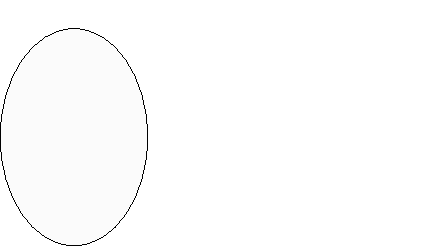
\includegraphics[width=\unitlength,page=1]{fig_shs.pdf}}%
    \put(0.09242613,0.24054801){\color[rgb]{0,0,0}\makebox(0,0)[lb]{\smash{$x_1$}}}%
    \put(0.12846631,0.36240699){\color[rgb]{0,0,0}\makebox(0,0)[lb]{\smash{$x_3$}}}%
    \put(0.13833525,0.11371431){\color[rgb]{0,0,0}\makebox(0,0)[lb]{\smash{$x_2$}}}%
    \put(0.92073981,0.50635972){\color[rgb]{0,0,0}\makebox(0,0)[lt]{\begin{minipage}{0.53112884\unitlength}\raggedright \end{minipage}}}%
    \put(0,0){\includegraphics[width=\unitlength,page=2]{fig_shs.pdf}}%
    \put(0.41093171,0.41327568){\color[rgb]{0,0,0}\makebox(0,0)[lb]{\smash{$\mathsmaller{\hash\left(x_3 \cat b\right) \mod 4}$}}}%
    \put(0.35,0.275){\color[rgb]{0,0,0}\makebox(0,0)[lb]{\smash{$\mathsmaller{\hash\left(x_1 \cat b\right) \mod 4}$}}}%
    \put(0,0){\includegraphics[width=\unitlength,page=3]{fig_shs.pdf}}%
    \put(0.81940596,0.29320931){\color[rgb]{0,0,0}\makebox(0,0)[lb]{\smash{$0\,1\,0\,0$}}}%
    \put(0.76349761,0.2128412){\color[rgb]{0,0,0}\makebox(0,0)[lb]{\smash{$\fprate = 2^{-4}$}}}%
  \end{picture}%
\endgroup%

    \caption{\emph{Singular Hash Set} over a \emph{countably infinite} universe}
    \label{fig:my_label}
\end{figure}


\subsection{Time and space complexity}
The probability that every element of $\Set{S}$ collides for a particular bit string in \cref{alg:ph} is given by the following theorem.
\begin{theorem}
The number of time steps the algorithm for $\shs(m,\fprate)$ is \emph{geometrically} distributed
\begin{equation}
	\RV{Q} \sim \geodist(\fprate^{m-1})
\end{equation}
 with an \emph{expected} number of steps given by
\begin{equation}
\label{eq:p_m_N}
	\fprate^{-(m-1)}\,.
\end{equation}
\end{theorem}
\begin{proof}
Suppose we have a set of bit strings $\Set{A} = \{b_1,\ldots,b_m\}$ and $b_1$ hashes to $y = \hash_k(b_1,n)$ where $\hash_k \colon \BitSet^{*} \mapsto \BitSet^k$ is a random hash function that uniformly distributes over its domain of $2^k$ possibilities.
Since $y$ is a particular element in $\BitSet^k$, the probability that $b_j$ for $j=2,\ldots,m$ hashes to $y$ is given by
\begin{equation}
    \frac{1}{2^k} = \fprate\,.
\end{equation}
Since $\hash_{\Set{S}}$ is a random hash function, the hashes of $b_1,\ldots,b_m$ are independent.
Thus, the joint probability that $b_2, \ldots, b_m$ hash to $y$ is given by the product of their marginal probabilities
\begin{equation}
    \fprate^{m-1}\,.
\end{equation}
\end{proof}

\begin{theorem}
The expected bit length of the Singular Hash Set obtains the information-theoretic lower-bound given by
\begin{equation}
    -\log_2 \fprate \; \si{bits \per element}\,,
\end{equation}
where $\fprate$ is the false positive rate.
\end{theorem}
\begin{proof}
Suppose $\Card{\Set{A}}=m$.
By \cref{alg:makeset}, $\shs_{\Fun{F} \Set{X}}(\Set{A},\fprate)$ is a value constructor that returns a pair of elements, $\Tuple{n',q}$ which has a bit length $\BL{n'} + \BL{q}$.
The bit length of $\BL{q}$ is just $-\log_2 \fprate$.
The bit length of $n'$ depends on the minimum value of $n$ found.

Computationally, we search in the order of increasing $n$, from $0$ to $\infty$.
The first case when a perfect collision occurs is a geometric distribution $\RV{Q} \sim \geodist \!\left(p = \fprate^{m-1}\right)$.
By \cref{def:mapping}, the $n$-th trial uniquely maps to a bit string of length $\lfloor \log_2 n \rfloor$.
Thus, the bit string has a random length given approximately by $\RV{N} = \log_2 \RV{Q}$ bits.
We approximate the logarithm with a second-order Taylor series around the \emph{expected} value of $\RV{Q}$ as given by
\begin{equation}
    \RV{N} \approx
        \log_2 \Expect{\RV{Q}} -
        \frac{\left(\RV{Q} - \Expect{\RV{Q}}\right)^2}{2 \Expect{\RV{Q}}^2}        
        \log_2 e\; \si{bits}\,.
\end{equation}
We are interested in the \emph{expected} value of $\RV{N}$,
\begin{equation}
\label{eq:proofspaceexplb}
    \Expect{\RV{N}} \approx
        \log_2 \Expect{\RV{Q}} -
        \frac{\Var{\RV{Q}}}{2 \Expect{\RV{Q}}^2} \log_2 e \; \si{bits}\,.
\end{equation}
The expectation and variance of $\RV{Q}$ is known to be $1/p$ and $(1-p)/p^2$ respectively, and thus we may rewrite \cref{eq:proofspaceexplb} as
\begin{equation}
\label{eq:proofspaceexplb2}
	\Expect{\RV{N}} \approx = -\log_2 p - \frac{1-p}{2} \log_2 e \; \si{bits}\,.
\end{equation} 
Substituting $\fprate^{m-1}$ for $p$ in \cref{eq:proofspaceexplb2} results in
\begin{align}
    \Expect{\RV{N}}
        &\approx -(m-1) \log_2 \fprate - \frac{1-\fprate^{m-1}}{2} \log_2 e \; \si{bits}\,.
\end{align}
In total, the bit length of $\Tuple{n',q}$ is thus
\begin{equation}
	\BL = -m \log_2 \fprate +  \frac{1-\fprate^{m-1}}{2} \log_2 e \; \si{bits}
\end{equation}
which asymptotically converges to $-\log_2 \fprate$ bits per element as $m \to \infty$.
\end{proof}

By \cref{eq:exp_trials}, \cref{alg:ph} has an expected time complexity that grows exponentially as $m$ grows The algorithm is intended to illustrate theoretical properties, not necessarily be used in practice.

\subsection{Probability distributions}
The bit representation of a singular hash set of $\Set{A}$ is uncorrelated with the specific elements of but is highly correlated with the its \emph{cardinality} $\Card{\Set{A}}$.



The probability that $\RV{B} = b$ is given by
\begin{equation}
\PDF{b \Given n}[\RV{B} \Given \RV{N}] = 2^{-n} \SetIndicator{\BitSet^n}(b)\,.
\end{equation}
\begin{proof}
Sketch proof.
\end{proof}




Given a false positive rate $\fprate$, the probability that $\RV{H} = h$ is given by
\begin{equation}
	\PDF{h \Given \fprate}[\RV{H}] = \fprate \, \SetIndicator{\BitSet^k}(h)\,,
\end{equation}
where $k = -\log_2 \fprate$.



\begin{theorem}
	The random bit length $\RV{N}$ has a probability mass function given by
	\begin{equation}
	\label{eq:N_pmf}
	\PDF{n \Given m, \fprate}[\RV{N}] = \left(\frac{1}{q}-q\right) q^{2^n} \SetIndicator{\NatSet}(n)\,,	
	\end{equation}
	where $q = 1 - \fprate^{m-1}$, $m$ is the cardinality of the objective set, and $\fprate$ is the false positive rate.
\end{theorem}
\begin{proof}
The probability that a bit string of length $n$ occurs is given by the probability that $\RV{Q}$ realizes some value in the range $\{2^n, \ldots, 2^{n+1}-1\}$, which is given by
\begin{align}
	\Prob{2^n-1 < \RV{Q} \leq 2^{n+1}-1}
		&= \Fun{F}[\RV{Q}]\!\left(2^{n+1}-1\right)-\Fun{F}[\RV{Q}]\!\left(2^n\right)\\
		&= \left(1-q^{2^{n+1}-1}\right) - \left(1-q^{2^n-1}\right)\\		
		&= q^{2^n-1} - q^{2^{n+1}-1}\,,
\end{align}
which is equivalent to the result.
\end{proof}

Given a false positive rate $\FPR = \fprate$ and an objective set of cardinality $m$, the joint distribution of $\RV{B}$, $\RV{H}$, and $\RV{N}$ is given by
\begin{equation}
\PDF{b,h,n \Given m,\fprate}[\RV{B},\RV{H},\RV{N}] = 2^{-n} \fprate \PDF{n \Given m,\fprate}[\RV{N}]\, \SetIndicator{\BitSet^n \times \BitSet^k \times \NatSet}(b,h,n)
\end{equation}
where $k = -\log_2 \fprate$.

In the singular hash set, the false positive rate and bit length $\RV{N}$ are \emph{observable}.
Therefore, a primary statistic of interest is the joint distribution of $\RV{B}$ and $\RV{H}$ given $\RV{N} = n$ and $\FPR = \fprate$, which is given by
\begin{equation}
\PDF{b,h \Given n,\fprate}[\RV{B},\RV{H} \Given \RV{N}] = 2^{-n} \fprate \, \SetIndicator{\BitSet^n \times \BitSet^k}(b,h)
\end{equation}
where $k = -\log_2 \fprate$.



%


The marginal distribution of $\RV{B}$ is given by marginalizing over the joint distribution with respect to $\RV{B}$, which yields the result
\begin{equation}
\PDF{b \Given \fprate, m}[\RV{B}] = 2^{-\BL(b)} \PDF{\BL(b) \Given m, \fprate}[\RV{N}]\,.
\end{equation}



A few key features of $\RV{B}$ is that it realizes the empty string with probability $\fprate^{m-1}$ and as $n$ goes to infinity, the probability that $\BL(\RV{B})=n$ goes to $0$.



NOTE: the singular hash set does not expose correlations by bit-wise operations, which may be a good thing, unlike in the bitwise models discussed previously.


%TODO: note that the SHS has a product type that is NOT UNIQUE. 
%Representational equality vs behavior equality, etc. Representationally, 
%different tuples may represent the exact same set, so representional 
%inequality 
%is not the same as behavioral equality. For any REGULAR FUNCTION, it should 
%not 
%matter which representation is given to the function as input, it should 
%produce the same output for any object that represents the same oblivious set.


The entropy of $\RV{N}$ is given by the following theorem.
\begin{theorem}
?
\end{theorem}
\begin{proof}
\begin{equation}
    \Entropy{\RV{N}} = -\Expect{\log_2 \PDF{\RV{N}}[\RV{N}]}\,.
\end{equation}

\begin{align}
    \Entropy{\RV{N}}
        &= -\sum_{n=0}^{\infty} \log_2 \PDF{n}[\RV{N}] \PDF{n}[\RV{N}]\\
        &= -\sum_{n=0}^{\infty} \log_2\! \left(q^{2^n-1}\left(1-q^{2^n}\right)\right) \PDF{n}[\RV{N}]\,.
\end{align}
\begin{equation}
\begin{split}
    \Entropy{\RV{N}}
        =&-\log_2 q \sum_{n=0}^{\infty}
            (2^n-1) \PDF{n}[\RV{N}] -\\
         &\sum_{n=0}^{\infty} \log_2\left(1-q^{2^n}\right) \PDF{n}[\RV{N}]\,.
\end{split}
\end{equation}

\begin{equation}
\begin{split}
    \Entropy{\RV{N}}
        =&-\log_2 q \left[\sum_{n=0}^{\infty}
            (2^n \PDF{n}[\RV{N}]\right] -\\
         &\sum_{n=0}^{\infty} \log_2\left(1-q^{2^n}\right) \PDF{n}[\RV{N}]\,.
\end{split}
\end{equation}
\end{proof}


\begin{theorem}
The random bit string that codes the singular hash set is a \emph{maximum entropy} coder for the \emph{approximate set} abstract data type.
\end{theorem}
\begin{proof}
The result immediately follows from the fact that the bit string is \emph{incompressible} and thus obtains maximum entropy.
The bit string $h_k \in \BitSet^k$ is, a priori, a random bit string uniformly distributed over $\BitSet^k$ by the property of the cryptographic hash function.
The bit string $b_n \in \BitSet*$ realizes a length $n$ with probability $\Fun{f}[\RV{N}](n)$.\footnote{As such, we can further compress $b_n$ using a geometric coder that assigns shorter bit strings to more probable lengths, but we require an \emph{in-place} bit string and so stick with the original code.}
Given $\RV{N}=n$, the bit string $b_n \in \BitSet^n$ is, a priori, a random bit string uniformly distributed over $\BitSet^n$.
\end{proof}

There are two predictable regularities in the bit string representation of a singular hash set.
\begin{enumerate}
	\item The \emph{randon bit length} $\RV{N}$ has relatively low entropy and is expected to obtain the information-theoretic lower-bound.
	\item The false positive rate has no uncertainty, i.e., zero entropy.
\end{enumerate}

By construction, we are able to estimate that an element is a member or non-member of $\Set{A}$ by determining if it is a member or non-member of $\OT{\PASet{A}}$, e.g., positive predictive value and other binary classification measures.

By construction, the singular hash set obtain the information-theoretic lower-bound, which may be used to estimte the cardinality of the objective sets being modeled by a singular hash set.
For instance, given a set $\Set{A}$, the random bit length $\RV{N}$ of bit string $b_n$ has a probability mass concentrated around the theoretical lower-bound.
Therefore, a \emph{method-of-moments} estimator of the cardinality of the $\Set{A}$ is given by
\begin{equation}
    \hat{\Card{\Set{A}}} = -\frac{\BL\!\left(\PASet{A}\right)}{\log_2 \fprate}\,,
\end{equation}
were $\BL$ is the bit length function and $\fprate$ is the \emph{false positive rate}.




\subsection{Relaxing optimality}
By \cref{dummy}, the time complexity is \emph{exponential} with respect to the cardinality $m$ of the objective set being modeled with a cipher set.
We can trade space complexity for time complexity to design more practical algorithms.

Let $\Set{A}$ be the objective set.
A general approach is to use a \emph{multi-level} hashing scheme such that each level generates smaller independent sub-problems.

We consider a two-level scheme.
At the first level, we find a hash function $\Fun{h}_k \colon \Set{X} \mapsto \{0,1,\ldots,k-1\}$ that maps $m/k$ elements in $\Set{A}$ to each element in the codomain.

\begin{definition}
The cryptographic $\alpha$-perfect hash function is a variation of the perfect hash function.
For each element in the codomain, proportion $\alpha$ of the domain maps to it.
\end{definition}

There are two degenerate cases to consider.
Suppose $\Set{A}$ is the objective set and $\Card{\Set{A}}=m$.
If $\alpha=1$, then it reduces to a \emph{singular} hash function where every element of $\Set{A}$ maps to the same value.
If $\alpha=\frac{1}{m}$, then it reduces to a \emph{minimal perfect hash function} of $\Set{A}$ where the hash function restricted to $\Set{A}$ is a bijection between $\Set{A}$ and $\{0,\ldots,m-1\}$.




The cryptographic $m/k$-perfect hash function has a space and time complexity given by the following theorem.
\begin{theorem}
A cryptographic $m/k$-perfect hash function has an expected space complexity given by
\begin{equation}
	-\alpha \log_2 \alpha
\end{equation}
and an expected time complexity given by
\begin{equation}
	\mathsmaller{\sqrt{\frac{k}{\alpha}}} \alpha^{\frac{k}{2}}
\end{equation}
where $\alpha \coloneqq \frac{m}{k}$.
\end{theorem}
\begin{proof}
Consider the family of hash functions of the type $\Set{X} \mapsto \{1,2,\ldots,k\}$.
When we restrict this family to some objective set $\Set{A}$ of cardinality $m$, we have hash functions of type $\Set{A} \mapsto \{1,2,\ldots,k\}$.
There are exactly $k^m$ hash functions of this type.

We are interested only in those hash functions of this type that evenly $k$-partition the domain into the codomain, i.e., the preimage of each element in the codomain consists of $\alpha \coloneqq m/k$ elements in the domain.

To count the number of possible functions, we choose $\alpha$ of the $m$ elements in the domain for element $1$ in the codomain.
There are a total of $m \choose \alpha$ ways of making this selection.
We remove these $\alpha$ elements from the domain.
We repeat the procedure again.
We choose $\alpha$ of the remaining $m-\alpha$ elements in the domain for element $2$ in the codomain.
There are a total of ${m-\alpha} \choose \alpha$ ways of making this selection.
If there are $a$ ways to make a first choice and $b$ ways to make a second choice, by the product rule there are $a b$ ways to make those two choices.
Thus, continuing this pattern, there are
\begin{equation}
	\prod_{j=1}^{k} {{m - j \alpha} \choose \alpha}
\end{equation}
ways to make the selections for the $k$ elements in the codomain, which simplies to
\begin{equation}
	\frac{m!}{(\alpha!)^k}\,.
\end{equation}

To generate perfect hash functions, we append some bit string to each input.
By the property of cryptographic hash functions, each bit string serves as an index into the cryptographic hash function family $\Set{A} \mapsto {0,1,\ldots,k-1}$.
Thus, since there are $k^m$ functions in this family in total, and only $\frac{m!}{(\alpha!)^k}$ $m/k$-perfect hash functions of this type, each time we index into the family, with probability
\begin{equation}
	p \sim e \mathsmaller{\sqrt{\frac{k}{\alpha}}} \alpha^{\frac{k}{2}}
%	p = \frac{m!}{(\alpha!)^k k^m}
\end{equation}
will the hash function be a $\alpha$-perfect hash function.

The probability of successfully finding an $m/k$-perfect hash function for each trial bit string is thus \emph{geometrically} distributed with a probability of success $p$.

The time complexity is just the \emph{expected} number of trials, which is $1/p$ for the geometric distribution, and the length of the successful bit string is just $\log_2 1/p$.
\end{proof}


\begin{figure}
\centering
\caption{The expected bits per element of the\\cryptographic $k$-perfect hash function.}
\begin{tikzpicture}
\begin{axis}[
axis lines = left,
	xlabel = $\alpha \coloneqq \frac{m}{k}$,
	ylabel = {$\mathcal{O}(-\alpha \log_2 \alpha)$},
]
\addplot [
	domain=-0:1, 
	samples=100, 
	color=blue,
]
{-log2(e)*x*log2(x) + x*ln(2*pi)};
\end{axis}
\end{tikzpicture}
\end{figure}


We employ the $m/k$-perfect hash function to construct a more practical variation of the singular hash set.

We $k$-partition the $m$ elements in a specified set using the $m/k$-perfect hash function, giving us $m/k$ elements per bin, and then we apply the singular hash set to each of these independently.

This is a negative binomial distribution.


Suppose we have two cryptographic hash functions, $\hash_1 \colon \BitSet^* \mapsto \BitSet^w$ and $\hash_2 \colon \BitSet^w \mapsto \BitSet^k$ where, in general, $w < k$ but this is not necessarily the case.
If $w >> \Card{\Set{A}}$, then the size of the cipher set is just $-w \log_2 \fprate$ where $\fprate = 2^{-k}$ since each element of $\Set{A}$, with high probability, maps to a unique hash by $\hash_1$.




The first-level hash function $\hash_k \coloneqq \Set{X} \mapsto \{0,1,\ldots,k-1\}$ is defined as
\begin{equation}
	\hash_{k}(x) \coloneqq \Tuple{h,n'}
\end{equation}
where
\begin{equation}
\begin{split}
	\phi(w,n) 	& \coloneqq \hash(n' \cat x') \mod k\,,\\
	\Set{Y}[l] 	& \coloneqq \SetBuilder{\phi(x,l) \in \BitSet^k}{x \in \Set{A}}\,,\\
	n 			& \coloneqq \min\left\{\SetBuilder{ j \in \NatSet }{ \Set{Y}[j] \in \PS{\BitSet^k} \land \Card{\Set{Y}[j]} = 1}\right\}\,.
\end{split}
\end{equation}





The first application of the cryptographic hash function maps each element to a particular index.
By the property of the cryptographic hash function, the elements are expected to be equally partitioned into the $k$ indices.
Next, at each index, we associate an independent bit string that serves the same purpose as the bit string $b_n$ in the singular hash set.
We then independently apply the singular hash set algorithm to each partition.
Let the number of trials necessary for singular hash set of the $j$-th partition be denoted by $\RV{T}_j$.
The total expected number of trials is just the sum of the geometrically distributed random variables $\RV{T} = \RV{T}_1 + \RV{T}_2 + \cdots + \RV{T}_k$, which is a \emph{negative binomial distribution},
\begin{equation}
	\RV{T} \sim \nbdist\left(k, \fprate^{\frac{m}{k}-1}\right)\,.
\end{equation}
%If a partition ends up being especially problematic, we may either increase $k$ or recursively subdivide the partition until a base case $k=1$ is trivial to solve.

The extra degree of freedom we have with the number of partitions $k$ means we can quantitatively trade space complexity for time complexity.
\begin{theorem}
The value of $k$ that is expected to yield a solution at $t$ trials is given by
\begin{equation}
	k = \alpha \Expect{\RV{N}}\,,
\end{equation}
where $\frac{1}{\alpha} = \log_2 \left(\frac{\fprate t}{k + t}\right)$.
\end{theorem}
\begin{proof}
We take the approach of solving for some $t$ number of trials and finding a lower-bound $k$ that satisfies the equation,
\begin{equation}
	\Expect{\RV{T}} = t\,.
\end{equation}
Substituting the expectation of the negative binomial into the above yields the equation
\begin{equation}
	\frac{k \fprate^{m/k-1}}{1-\fprate^{m/k-1}} = t\,.
\end{equation}
Solving for $k$ yields the result.
\end{proof}

We know that, approximately, the bit length is given by
\begin{equation}
	\RV{N} = \log_2 \RV{T}\,,
\end{equation}
which may be solved as described in \cref{dummy}.

We may also quantify the probability that, after $t$ trials, some jointly chosen value of $k$, $t$, and $\fprate$ fails to realize a solution.
In fact, we can quantify the probability that $r$ of the $m$ elements fails, which yields a \emph{rate-distortion} $\frac{r}{m}$.

If after $t$ trials no solution is found, we may either continue with the search or stop short, resulting in not just an approximate set with \emph{false positives} but also \emph{false negatives}.
We refer to this outcome as a \emph{rate-distorted set}, where the rate distortion is a function of time.
However, note that we could also make the rate-distortion a function of \emph{space}, i.e., limit the maximum size of the bit string code and choose the code that yields the smallest false negative rate.


If we are interested in rate-distorted sets with false negative rates greater than $0$, then an alternative approach is to consider the probability of failure for a particular $k$, $\fprate$, and $m$.
By the survival function of the negative binomial, the probability that more than $t$ trials (or $\log_2 t$ bits) is required for a particular parameterization $k$ and $p = \fprate^{\frac{m}{k}-1}$ is given by
\begin{equation}
	\Fun{I}[p](t+1, k)\,,
\end{equation}
where $\Fun{I}[p]$ is the \emph{regularized incomplete beta function}.





\begin{theorem}
	A value of type $\SHS_{\Set{X}}^{k}$ constructed with $\shs_{\Set{X}}(\Set{A},\fprate \; \Given \; k = m)$ \emph{models} a cryptographic perfect hash function $\hash_{\Set{A}} \colon \Set{X} \mapsto \{0,1,\ldots,-\log_2 \fprate\}$ where $\Set{A} \subseteq \Set{X}$ and $r = \frac{\Card{A}}{-\log_2 \fprate}$.
\end{theorem}



\subsection{Boolean algebra}
The data structure does not trivially model a Boolean algebra with simple bit-wise operators on its representation, as is the case with $\Fun{F}$ and $\Fun{G}$, but it may be \emph{lifted} to a Boolean algebra by the fact that
\begin{equation}
\Set{A} \SetUnion \Set{B} = \SetBuilder{x \in {\Set{X}}}{x \in \Set{A} \lor x \in \Set{B}}
\end{equation}
and other similar identities.
Specifically, we define a \emph{recursive} type for the Boolean algebra as
\begin{align}
\Fun{B}_{\OT{\Set{X}}} \coloneqq & \, \Btm_{\OT{\Set{X}}} + \Top_{\OT{\Set{X}}} \\
+ & \Fun{Just} \SHS_{\OT{\Set{X}}} \\
+ & \Fun{Join} \, \Fun{B}_{\OT{\Set{X}}} \, \Fun{B}_{\OT{\Set{X}}} \\
+ & \Fun{Meet} \, \Fun{B}_{\OT{\Set{X}}} \, \Fun{B}_{\OT{\Set{X}}} \\
+ & \Fun{Not}  \, \Fun{B}_{\OT{\Set{X}}} \,.
\end{align}

Then, for instance, set-union $\SetUnion \colon \Fun{B}_{\OT{\Set{X}}} \times \Fun{B}_{\OT{\Set{X}}} \mapsto \Fun{B}_{\OT{\Set{X}}}$ is defined as $a \SetUnion b \coloneqq \Fun{Join} a \, b$.

Over the Boolean algebra $\Fun{B}_{\OT{\Set{X}}}$, the membership predicate
\begin{equation}
\SetContains \colon \Fun{B}_{\OT{\Set{X}}} \times \Fun{B}_{\OT{\Set{X}}} \mapsto \BitSet
\end{equation}
is defined as
\begin{align}
x \SetContains \Top_{\OT{\Set{X}}} 	& \coloneqq 1\,,\\
x \SetContains \Btm_{\OT{\Set{X}}} 	& \coloneqq 0\,,\\	
x \SetContains \Fun{Just} a		   	& \coloneqq x \SetContains a\,,\\
x \SetContains \Fun{Join} a \, b 	& \coloneqq \left(x \SetContains a\right) \lor
\left(x \SetContains b\right)\,,\\
x \SetContains \Fun{Meet} a \, b 	& \coloneqq \left(x \SetContains a\right) \land
\left(x \SetContains b\right)\,,\\
x \SetContains \Fun{Not} a		 	& \coloneqq \neg \left(x \SetContains a\right)\,.
\end{align}

The nature of the composition reveals something about the sets and decreases entropy.

With respect to the above, any Boolean algebra
\begin{equation}
A \coloneqq \left(\PS{\Set{X}}, \SetUnion, \SetIntersection, \SetComplement, \EmptySet, \Set{X}\right)\,.
\end{equation}
may be mapped to the Boolean algebra
\begin{equation}
B \coloneqq \left(\Fun{B}_{\OT{\Set{X}}}, \SetUnion, \SetIntersection, \SetComplement, \Btm_{\OT{\Set{X}}}, \Top_{\OT{\Set{X}}}\right)\,.
\end{equation}
Interestingly, the mapping from $A$ to $B$ is not a homomorphism since, for instance, $\shs_{\OT{\Set{X}}}(\Set{A}) \SetUnion \shs_{\OT{\Set{X}}}(\Set{B})$ does not necessarily equal $\shs_{\OT{\Set{X}}}(\Set{A} \SetUnion \Set{B})$ due to the random approximate set model.
That is, the mapping only \emph{probabilistically} preserves relations according to the \emph{higher-order} random approximate set model.
One might say that it is \emph{asymptotically} homomorphic $(\fprate \to 0)$.






\emph{Rate-distorted cipher set}
The \emph{false positive rate} of an approximate cipher set is a \emph{rate-distortion}.
The rate distortion is a function of strictly space constraints.

We consider another kind of rate distortion that generates \emph{false negatives} which is either a function of space or time constraints.

The result is an approximate cipher set with both a first-order false positive \emph{and} false negative rates.
Note that cipher sets with higher-order false negatives and false positives may also be generated by \emph{composing} the cipher sets, but here we consider a value constructor of cipher sets that generates first-order approximation errors.

The number of elements that collide on the \emph{singular hash} on any particular trial is binomially distributed,
\begin{equation}
	\RV{T} \sim B(m-1,p)
\end{equation}
where $p = \fprate$.
When we are only interested in $m$ `successes', the probability is given as before, $\fprate^{m-1}$.

There are a few different ways of treating the rate distortion $\fnrate$ and $\fprate$.

We consider the false positive rate $\fprate$ first.
Generally, we specify a value that is a compromise between space and accuracy.
Since the cost of a false positive and the cost of a false negative may differ, different values for each may be preferable.

One way is to treat $\alpha$ as a random variable that is induced by a maximum bit rate per element, e.g., on average the maximum number of bits per element is $b$.
Thus, if there are $m$ elements, the constructor is limited to finding a bit string of length $b m$.

Another way to proceed is to say that we are satisfied with proportion $(1-\alpha)$ elements or more being perfectly hashed.


\end{document}  